\begin{frame}
    \frametitle{Conclusion}
    Cyclus is a performant, expanding fuel cycle simulator that holds promise for future applications. It demonstrated its capability to:
    \begin{itemize}
        \item `Predict the past'
        \item Model transition scenarios
        \item Visualize important fuel cycle metrics
    \end{itemize}
\end{frame}

\begin{frame}
    \frametitle{Future Work Ongoing}
    \texttt{Cycamore} is adequate for rough analyses, but more accurate
    modules or additional tools would increase analysis fidelity
    \begin{itemize}
        \item Dynamic archetype parameters (e.g. \texttt{refuel\_time}
                changing in time or sampled from a distribution)
        \item In-module depletion (i.e. Using in-module SERPENT Reduced-order-model)
        \item Demand-driven deployment \footnotemark
        \item Database-based MSR simulator
    \end{itemize}
    \footnotetext{NEUP 16-10512}
\end{frame}


\begin{frame}
    \frametitle{Room for Improvement}
    To really take it to the next level, a more organized, supported
    effort is needed.
    \begin{itemize}
        \item Organized / Supported Code development and Quality Assurance (QA)
        \begin{itemize}
            \item Currently done by a Cylcus Community Manager (25\% PostDoc)
            \item User support and bug fixing on Github done
            \item Various archetypes are outdated
        \end{itemize}
        \item Easier User Interface (UI) for broader user base
        \begin{itemize}
            \item Input generation / validation / visualization (e.g. Fulcrum)
            \item Ouput visualization / postprocessing (e.g. ORION)
        \end{itemize}
    \end{itemize}
\end{frame}


\begin{frame}
    \frametitle{Why \Cyclus?}
    \Cyclus has a unique expandable nature due to its open-source-ness and
    modularity of models. Here are potential projects with Cyclus:
    \begin{itemize}
        \item Central database driven high fidelity fuel cycle simulation
        \begin{itemize}
            \item Every fuel cycle facility in the Evaluation and Screening report modeled
            \item Real-life designs (Reactor designs, Reprocessing technologies etc.)
            \item plug-and-play for user
        \end{itemize}
        \item GIS-based work (every agent can have a coordinate property)
        \begin{itemize}
            \item Transportation model
            \item Energy demand / region based deployment (i.e. EAGLE-I)
        \end{itemize}
        \item Various Metrics Connector
        \begin{itemize}
        	\item Postprocessor for Safeguard / Non-proliferation metrics
        \end{itemize}
        \item Cyclus is a good tool for comparison studies for different types of electrical generation or co-generation (Expandable to other systems)
    \end{itemize}
\end{frame}


\begin{frame}
	\frametitle{Synergy with ORNL}
	\begin{itemize}
        \item Archetypes of different models (Collective toolset)
		\item Most importantly: the personnel resources
		\item Fuel Cycle simulation is a combination of all aspects of nuclear engineering
		\item Insight / data from Safeguards, Reactor Physics
		\item Engage in discussion of questions that needs to be answered
	\end{itemize}
\end{frame}


\begin{frame}
	\frametitle{Synergy with ORNL}
	\begin{itemize}
		\item \Cyclus is a tool. It should be developed to fulfill the needs of its stakeholders.
		\item ORNL is an awesome resource for those interesting questions and insight.
	\end{itemize}
\end{frame}


\begin{frame}
	\frametitle{Conclusion II}
	\begin{itemize}
		\item \Cyclus, with partnership with ORNL, can become a one-stop tool for system integration analysis.
        \item To achieve this, sustained engagement with ORNL is needed for \Cyclus
        \item Size of a community is directly proportional to its sustainability
		\item Staff can `plug in' their developed model (reactor design, fuel cycle facility etc) to see the model's performance in a larger system.
	\end{itemize}
\end{frame}




\begin{frame}
    \frametitle{Acknowledgements}
    Invaluable advice and help provided by:
    Joshua Peterson-Droogh, Kathryn Huff, Andrew Worrall, Eva Davison, and Robert Flannagan
    \hfill \break
    \hfill \break
    The EU work has been performed using funding received from the DOE Office of Nuclear Energy's Nuclear Energy University Program (Project 16-10512) 'Demand-Driven Cycamore Archetypes'.
    \hfill \break
    \hfill \break
    This summer sponsored by:
    NESLS program at ORNL

\end{frame}

\begin{frame}
    Thank you. Questions / Concerns / Ideas?
\end{frame}


\begin{frame}
    \frametitle{My vision - Central Database}
    Central database driven high fidelity fuel cycle simulation
    \begin{itemize}
        \item Every fuel cycle facility in the Evaluation and Screening report modeled
        \item Real-life designs (Reactor designs, Reprocessing technologies etc.)
        \item plug-and-play for user
    \end{itemize}
    Example:
    \begin{itemize}
        \item reactor geometry, fuel composition, depletion calculation results
        \item journal articles published related to design (web scraping)
        \item archived physics calculations related to design
    \end{itemize}
\end{frame}


\begin{frame}
    \frametitle{My vision - Central Database}
    \begin{itemize}
        \item Leverage ORNL resources
        \begin{itemize}
            \item Reactor Physics Data / Results
            \item Export Control Infrastructure
            \item Stable funding
        \end{itemize}
        \item Build structured, referenced, central database
        \begin{itemize}
            \item the database would be controlled
            \item couple it to Cyclus for system integration analysis
            \item Can be used for other fuel cycle simulator
            \item Can be used for other general purposes (informational website)
        \end{itemize}
    \end{itemize}
\end{frame}

\begin{frame}
    \frametitle{Rough Coupling}
    \begin{itemize}
        \item Direct Coupling causes export control issues
        \item Larger maintenance with framework development
        \item Use reactor design's `interaction with outside' as data
        \begin{itemize}
            \item e.g. fuel in / out of reactor
        \end{itemize}
        \begin{figure}[htbp!]
        \begin{center}
        \centering
                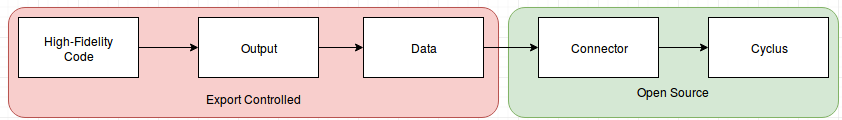
\includegraphics[width=\textwidth]{./images/con.png}
        \end{center}
    \end{figure}
    \end{itemize}
\end{frame}